% v2-acmlarge-sample.tex, dated March 6 2012
% This is a sample file for ACM large trim journals
%
% Compilation using 'acmlarge.cls' - version 1.3, Aptara Inc.
% (c) 2011 Association for Computing Machinery (ACM)
%
% Questions/Suggestions/Feedback should be addressed to => "acmtexsupport@aptaracorp.com".
% Users can also go through the FAQs available on the journal's submission webpage.
%
% Steps to compile: latex, bibtex, latex latex
%
%\documentclass[prodmode,acmtap]{acmlarge}
\documentclass[10.5pt]{article}

\addtolength{\voffset}{-50pt}
\addtolength{\hoffset}{-50pt}
\addtolength{\textwidth}{100pt}
\addtolength{\textheight}{100pt}

%\usepackage[a4paper,pdftex]{geometry}
\usepackage[utf8x]{inputenc}
\usepackage[italian]{babel}
\usepackage{makeidx}
\usepackage{graphicx}

\linespread{1.1}

% Package to generate and customize Algorithm as per ACM style
%\usepackage[ruled]{algorithm2e}
%\SetAlFnt{\algofont}
%\SetAlCapFnt{\algofont}
%\SetAlCapNameFnt{\algofont}
%\SetAlCapHSkip{0pt}
%\IncMargin{-\parindent}
%\renewcommand{\algorithmcfname}{ALGORITHM}

% Title portion
\title{RoundWord\\
\large{Progetto per il Corso di Sistemi Distribuiti, a.a. 2012-2013}}
\author{MATTEO BRUCATO e MIRO MANNINO\\Università di Bologna}


\begin{document}
%\large

\maketitle

\begin{abstract}
% (non più di dieci righe): riassume di cosa tratta la relazione.

\end{abstract}


\tableofcontents

\section{Introduzione}
% in cui si inquadra il problema affrontato, chiarendo gli obiettivi, riassumendo lo stato dell'arte, e descrivendo la struttura della relazione.

La presente relazione tratta della realizzazione del progetto per il corso di sistemi distribuiti, dalla sua ideazione, alle scelte progettuali, agli aspetti implementativi, non senza includere difficoltà incontrate e ciò che abbiamo imparato da questa esperienza formativa.

Un gioco molto famoso tra i bambini di ogni età, ma giocato anche tra adulti senza limiti di età, consiste nel formare sequenze di parole collegate tra di esse attraverso sillabe. Il gioco è molto semplice e non richiede nessuna strumentazione né attrezzature particolari, e può esser giocato in qualunque contesto. Per giocare, basta avere una comune conoscenza del vocabolario italiano ed essere in grado di suddividere le parole in sillabe. 

%Io direi di mettere un limite...
%Può essere giocato da un numero minimo di due giocatori, e non vi è un limite massimo.

Non essendo a conoscenza del nome del gioco (nonostante lo abbiamo giocato sin da bambini), abbiamo deciso di chiamarlo \emph{RoundWord} per il presente progetto.

\begin{figure}
	\begin{center}
		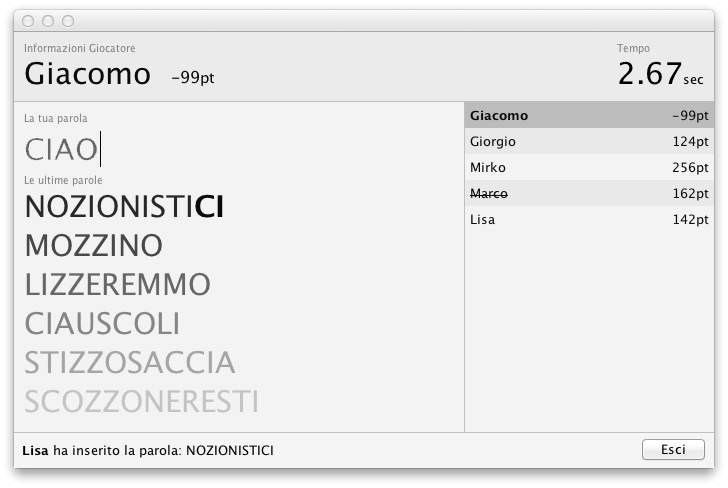
\includegraphics[scale=0.5]{imgs/screenshot.png}
		\caption{Una screenshot del gioco dove Giacomo detiene il turno e pertanto deve inserire una parola. Notare anche che Marco si è ritirato, oppure ha avuto un crash.}
	\end{center}
\end{figure}


\subsection{Regole del gioco}
All'inizio del gioco, i giocatori decidono di comune accordo una sequenza di gioco, ovvero l'ordine dei turni (giocando dal vivo, ci si mette spesso in cerchio). Ogni giocatore, al proprio turno, produrrà una singola parola. Il primo giocatore sceglie una parola qualunque, che deve essere \emph{presente nel dizionario} italiano utilizzato dal gioco. Dal secondo giocatore in poi, scatta la regola per la scelta della parola:

\begin{itemize}
\item Sia $w$ la parola prodotta dal giocatore precedente. Ad esempio ``VERIFICA''.
\item Sia $w=w_1, w_2, \dots, w_n$ la sua suddivisione in sillabe. Ad esempio, ``VE'', ``RI'', ``FI'', ``CA''.
\item Sia $w'=w'_1, w'_2, \dots, w'_m$ la parola inserita dal giocatore corrente, e la sua suddivisione in sillabe.
\item La parola $w'$ è \emph{valida} se è presente nel dizionario e se $w_n = w'_1$, ovvero se la prima sillaba della nuova parola è uguale all'ultima sillaba della parola precedente. Ad esempio, ``CARI'' e ``CARATTERISTICA'' sono tutte parole valide, mentre ``CARTA'', ``RESPIRARE'' e ``MANO'' sono tutte parole non valide.
\end{itemize}

Ciò quindi crea una sequenza di parole tutte collegate tra di esse per mezzo dell'ultima e della prima sillaba tra ogni coppia di parole. 

Per rendere più interessante il gioco, non basta che una parola sia \emph{valida} affinché si possano guadagnare dei punti per il proprio turno. Vi è un altro requisito fondamentale: la parola deve essere \emph{nuova}. Ovvero, la parola inserita non deve essere stata inserita precedentemente da alcun giocatore, durante il corso della corrente partita. Quindi, ogni giocatore deve tenere memoria della sequenza di parole generate da tutti i giocatori, ed evitare di riproporre una parola già inserita precedentemente. Per aiutare l'utente a capire le parole che sono state inserite, vengono visualizzate le ultime 6 parole.

Per complicare ulteriormente il gioco, e per evitare che il gioco duri troppo, ogni giocatore ha un limite di tempo entro il quale può proporre la sua parola.

Ogni giocatore, al proprio turno, può guadagnare o perdere punti, secondo le seguenti regole:
\begin{itemize}
\item Se la parola non è presente nel dizionario perde 80 punti.
\item Se la parola non è valida perde 80 punti.
\item Se la parola è \emph{valida}, ma non è \emph{nuova}, perde 50 punti.
\item Se il giocatore non è riuscito a produrre la parola entro il limite di tempo stabilito per un singolo turno, perde 100 punti.
\item Se la parola è valida e non è stata proposta precedentemente durante la stessa partita, il giocatore guadagna un numero di punti che dipende dalle lettere utilizzate, in base alla distribuzione delle lettere nelle parole italiane (e.g. 1 punto per la lettera A, 8 per la lettera G), dalla lunghezza della parola (i.e. 5 punti in più per ogni lettera inserita dopo la quinta), e dai millesimi di secondo impiegati (i.e. 0.02 punti per ogni millisecondo che l'utente aveva ancora a disposizione per rispondere).
\end{itemize}

Da notare che, nel caso un giocatore perda dei punti durante il proprio turno, la parola proposta non viene aggiunta alla lista delle parole utilizzate, il prossimo giocatore dovrà pertanto riprendere dalla parola dell'ultimo giocatore che era riuscito ad inserire una parola valida e nuova.

Un giocatore può ritirarsi in qualunque momento. In quel caso, il gioco continua tra i giocatori rimanenti, richiudendo il cerchio nella maniera naturale. Il gioco finisce quando un giocatore rimane da solo, oppure quando nessun giocatore riesce a produrre parole valide e nuove per un intero ciclo di gioco. Nel primo caso, il vincitore è l'unico ``superstite''. Nel secondo caso è quello con il punteggio maggiore tra i giocatori superstiti.

\subsection{Obiettivi del progetto}

L'obiettivo principale del presente progetto è la realizzazione del gioco in un ambiente distribuito, in cui varie entità distribuite (che chiameremo \emph{peer}, vista la loro intrinseca natura client/server) comunicano tra loro attraverso una rete asincrona, non affidabile, come quella di Internet. In questo tipo di contesto sono necessari coordinazione tra i peer e gestione di stati condivisi. Infatti, lo stato del gioco, composto di elementi che devono essere condivisi tra i vari peer in maniera coerente, non può risiedere in un unico peer che funge da nodo centrale.

Sono state fatte delle semplificazioni per non dovere affrontare errori difficili da risolvere, che sono le stesse riportate dalle specifiche del progetto: per prima cosa si assume di avere delle comunicazioni affidabili (ovvero non è possibile che si guastino), ed i processi possono avere solamente guasti di tipo crash. Ciò significa che assumiamo sempre che un peer che non riusciamo a contattare, per un certo periodo di tempo, sia un peer che ha subito un crash, piuttosto che un peer che non riusciamo a contattare per via di un fallimento della rete, o per via di una temporanea indisponibilità del peer stesso. 

Alcuni problemi correlati a queste assunzioni sono comunque stati risolti. Si pensi ad esempio che un peer che precedentemente dichiarato crashato, poiché lento o per ritardi di comunicazione, torna a comunicare con i peer della rete, viene comunque ignorato: il giocatore vedrà un messaggio che lo avverte del fatto che la propria connessione è troppo lenta e che quindi è stato cacciato fuori la partita, come avviene in molti giochi commerciali.

Inoltre, secondo le specifiche, come paradigma di comunicazione, è stato utilizzato remote invocation, in particolare il Remote Method Invocation (RMI) di Java. Ciò fornisce un modo semplice ed ad alto livello per comunicare tra i vari peer, che ha semplificato molto l'implementazione delle comunicazioni tra di essi, in quanto tale middleware permette di mascherare l'eterogeneità tra le varie macchine. Ciononostante non è sufficiente da solo per fornire tutte le funzionalità di un ambiente distribuito, come la coordinazione, la gestione degli errori e del tempo.

\section{Aspetti progettuali}
% in cui si illustra il progetto svolto; in particolare si discutono i problemi specifici affrontati, le soluzioni valutate e proposte, e l'architettura astratta del sistema sviluppato.

\subsection{Interpretare RoundWord come un sistema distribuito}
Interpretare questo gioco nell'ambito dei sistemi distribuiti non è particolarmente difficile. Infatti, ogni giocatore è controllato da un \emph{peer}, in una rete distribuita in stile peer-to-peer (senza overlay). I turni a ciclo suggeriscono l'idea di un protocollo in stile \emph{token-ring}, dove il detentore del turno viene equiparato al \emph{leader} attuale, e la leadership viene passata al prossimo peer allo scadere di ogni turno (per questo motivo ci riferiremo a \emph{leader}, \emph{detentore del turno} o \emph{coordinatore} come sinonimi). Lo \emph{stato condiviso} tra i peer partecipanti consiste in:
\begin{itemize}
\item La lista dei peer (crashati e non crashati).
\item La lista dei punteggi dei rispettivi giocatori.
\item La lista completa delle parole inserite dai giocatori.
\item L'identità del detentore del turno attuale (ovvero del leader attuale).
\end{itemize}


\subsection{Architettura astratta}

\begin{figure}
\centering
\includegraphics[scale=1]{imsg/architettura-astratta.pdf}
\caption{Architettura astratta del sistema}
\label{img:architettura-astratta}
\end{figure}

Il sistema, a livello astratto, è composto da tre componenti principali ben distinte tra loro: (1) il \emph{modello del gioco}, (2) il \emph{controllore dei giocatori} e (3) il \emph{modulo di comunicazione}. Le tre componenti sono rappresentate in Figura~\ref{img:architettura-astratta}.

La parte di modellazione del gioco racchiude a sua volta tutte le componenti che modellano il gioco, come ad esempio il tavolo di gioco, i giocatori e la gestione delle parole del dizionario.
Questo modulo ignora il fatto che il gioco venga eseguito in rete o in locale, con utenti reali o intelligenze artificiali.
Pertanto, esso fornisce solamente dei metodi per cambiare lo stato del gioco, e genera eventi per segnalare tali cambiamenti.

Il controllore dei giocatori gestisce le azioni dei giocatori e ne riporta le scelte sul modello di gioco. Per semplicità (e per maggior divertimento) abbiamo previsto che il gioco possa essere giocato sia da utenti reali che da intelligenze artificiali (AI). Una semplice AI è stata anche realizzata nel corso del progetto. Il controllore può essere quindi di due tipi: una GUI, per chiedere e ricevere input dall'utente e fornirgli output, e una AI, che simula le azioni di un giocatore ``reale''.
%possono essere di tre tipi: un'interfaccia grafica che comunica con il giocatore reale permettendogli di poter giocare, un peer remoto che interagisce sfruttando la parte di comunicazione, o un giocatore automatico (principalmente utilizzato per debug, ma che comunque non si esclude possa essere utilizzato come un rimpiazzo per i giocatori che hanno subito un guasto).

Il modulo di comunicazione è la parte centrale del sistema distribuito, in quanto gestisce l'interazione tra i peer del sistema. I compiti principali di questo modulo sono quelli di permettere lo scambio dei messaggi del gioco (le nuove parole inserite dai giocatori), la gestione dello stato condiviso e l'implementazione dei protocolli di gestione dei guasti di tipo crash.
%Ogni peer ha il compito di gestire un particolare giocatore, eseguendo delle azioni opportune per ogni tipo di evento generato dal gioco.
Ogni peer gestisce gli eventi generati dal giocatore locale e dai giocatori remoti, eseguendo di volta in volta le azioni opportune.

Per gestire le comunicazioni con gli altri peer, il modulo è suddiviso in due sotto-moduli: uno che funge da client (chiamato \emph{client side}) e uno che funge da server (chiamato \emph{server side}). Il client side gestisce i messaggi in uscita (non è altro che un thread fornito di una coda di messaggi), mentre il server side gestice i messaggi in entrata ed esegue tutte le azioni opportune, in base al tipo di messaggio ed ai dati in esso contenuti. 
Ad esempio, per gestire l'evento del giocatore locale che ha inserito una parola, un peer crea un messaggio specificando il peer destinatario e lo pone in uscita aggiungendolo semplicemente alla coda di messaggi in uscita del proprio client side; successivamente, tale messaggio verrà processato e inviato chiamando l'opportuna funzione del server side del peer destinatario.


\subsection{Protocolli distribuiti}
Nel seguito, descriveremo i protocolli di comunicazione e interazione distribuita facenti parte del modulo di comunicazione.

\subsubsection{Inizializzazione della partita}

La procedura di inizializzazione della partita utilizza un server centrala ed è l'unica procedura del gioco che prevede componenti centralizzate. Tale scelta, oltre che essere prevista nelle specifiche, è un'importante semplificazione che elimina il bisogno di complicate procedure di discovery distribuite. Ma è anche un'assunzione realistica e molto usata in parecchi giochi commerciali.

Il server centrale, chiamato \textit{registrar}, è un server HTTP che provvede a raccogliere gli indirizzi IP e le porte dei vari peer che vogliono giocare, ed i nickname dei relativi giocatori. Tale server viene configurato in esecuzione per creare partite di $N$ giocatori, e quindi dà il via libera solo dopo che sono state fatte $N$ richieste proveniente da altrettanti giocatori differenti.

Al momento del raggiungimento delle $N$ richieste, il registrar manda, ad ogni giocatore, la lista degli utenti (e relativi peer) che parteciperanno alla partita. Tale lista $[p_1, p_2, .., p_N]$ è ordinata ed identica per tutti, stabilendo quindi quale sarà l'ordine con il quale avverranno i turni di gioco. Ogni lista di giocatori arriva ai vari peer in momenti differenti, e per questo motivo è necessario che tutti i peer siano a conoscenza del fatto che tutti gli altri l'abbiano già ricevuta prima di poter iniziare la partita. Se così non fosse il peer che detiene il turno, iniziando a giocare, potrebbe assumere falsamente che alcuni peer abbiano subito un guasto. Il peer che deve per primo iniziare a giocare (ha il turno), invia pertanto un messaggio di \textit{Hello}, attendendo che questo ritorni indietro. Nel caso in cui tale messaggio non dovesse ritornare (si utilizza un timeout), la partita viene annullata, per fare sì che se ne possa ricreare una nuova. 

\subsubsection{Comunicazione}

Da notare, dalla descrizione della parte di comunicazione, che c'è un disaccoppiamento tra il peer e l'invio dei messaggi. Questo perché, per implementare il progetto, è stato utilizzato il paradigma di invocazione a metodo remoto, in particolare \textit{Java RMI}. Inviare un messaggio equivale pertanto ad eseguire una funzione in un oggetto remoto: nel nostro caso è il client side ad eseguire la funzione nel server side del destinatario. Detto ciò è stato deciso di creare un thread separato (il client side) che si occupasse solo dell'invio dei messaggi, in modo da non bloccare l'intera applicazione per lunghi periodi (si pensi all'attesa causata da un peer che non risponde, oppure ad un messaggio che altro non è che una chiamata ricorsiva). In tal modo, il peer che deve solamente fare un forward a $P_2$ del messaggio proveniente da un peer $P_1$, all'interno del metodo nel server side (invocato da $P_1$), creerà un messaggio analogo a quello generato da $P_1$, cambiando solamente il destinatario, ed incodandolo al proprio client side, con il risultato che il client side di $P_1$ termina immediatamente, senza aspettare che $P_2$ riceva il messaggio. 




\section{Aspetti implementativi}
% dettagli sulle scelte implementative, ed architettura specifica implementata. Inserire almeno il diagramma delle classi e uno delle interazioni secondo lo standard UML.

\subsection{Architettura}

\subsubsection{Modellazione del gioco}

Il gioco in sé viene rappresentato da poche classi: \texttt{GameTable}, \texttt{Word}, \texttt{Player} e \texttt{Dictionary}.

La classe \texttt{Word} rappresenta una parola del gioco. Consiste di una semplice stringa, ma ha numerosi metodi utili per scomporla in sillabe e determinarne il valore in punteggi. Inoltre essa è serializzabile, poiché deve poter essere inviata lungo la rete.  

La classe \texttt{Dictionary} rappresenta un dizionario, e contiene semplici metodi per il lookup di una parola.

La classe \texttt{Player} rappresenta un giocatore. Esso ha un nickname, un punteggio, uno stato (attivo o non attivo), ed altre informazioni necessarie per il gioco. Esso può essere controllato da un giocatore reale presente sullo stesso peer, da un agente che gioca automaticamente, oppure controllato un peer remoto.

La classe \texttt{GameTable} rappresenta il tavolo di gioco. Essa contiene informazioni quali: la lista delle parole che sono state inserite, come anche la lista dei giocatori, ed il giocatore che detiene il turno. Inoltre ha dei metodi per modificare lo stato del gioco, come quello per determinare chi è il prossimo detentore del turno, o per inserire una nuova parola. Tale classe non ha un'idea del fatto di come viene controllato un giocatore; seguendo il design pattern chiamato \textit{Observer Pattern}, la classe è stata progettata per generare degli eventi, quali ad esempio l'inserimento di una nuova parola, il cambio del turno, o la terminazione del gioco. Sono poi presenti diversi listener che rispondono in maniera passiva a questi eventi seguendo delle azioni opportune. Queste stesse entità che fungono anche da listener, possono comunque avere dei ruoli attivi, come ad esempio l'inserimento di nuove parole. 

L'entità più semplice, chiamata \texttt{FakePlayer}, che rappresenta un agente che gioca automaticamente, consiste ad esempio in un semplice loop, che inserisce una parola, e che rimane in attesa fin tanto che il \texttt{GameTable} non genera un evento, in modo da segnalare che tale agente è il detentore del prossimo turno. 

Al contrario, un giocatore reale ha tanti oggetti, che rappresentano varie componenti dell'interfaccia. Ognuno di essi può fungere anche da listener, in modo da poter aggiornare le varie informazioni che gli competono. Inoltre, l'interfaccia ha anche un ruolo attivo, poiché inserisce le parole che sono state scritte dall'utente, calcolando anche il tempo impiegato per farlo.

Più complicato è invece un giocatore controllato da un peer remoto. Il \texttt{Peer}, che funge anche da listener, può reagire ad un evento, quale ad esempio l'inserimento di una nuova parola, mandando dei messaggi per informare anche agli altri peer di tale evento. Può poi inserire nuove parole sulla base dei messaggi ricevuti dagli altri peer, cambiare lo stato di un giocatore (ad esempio a causa di un crash), oppure decidere chi possederà il prossimo turno in base sullo stato degli altri peer.

\begin{figure}
	\vspace*{-1in}
	\begin{center}
		\hspace*{-0.5in}
		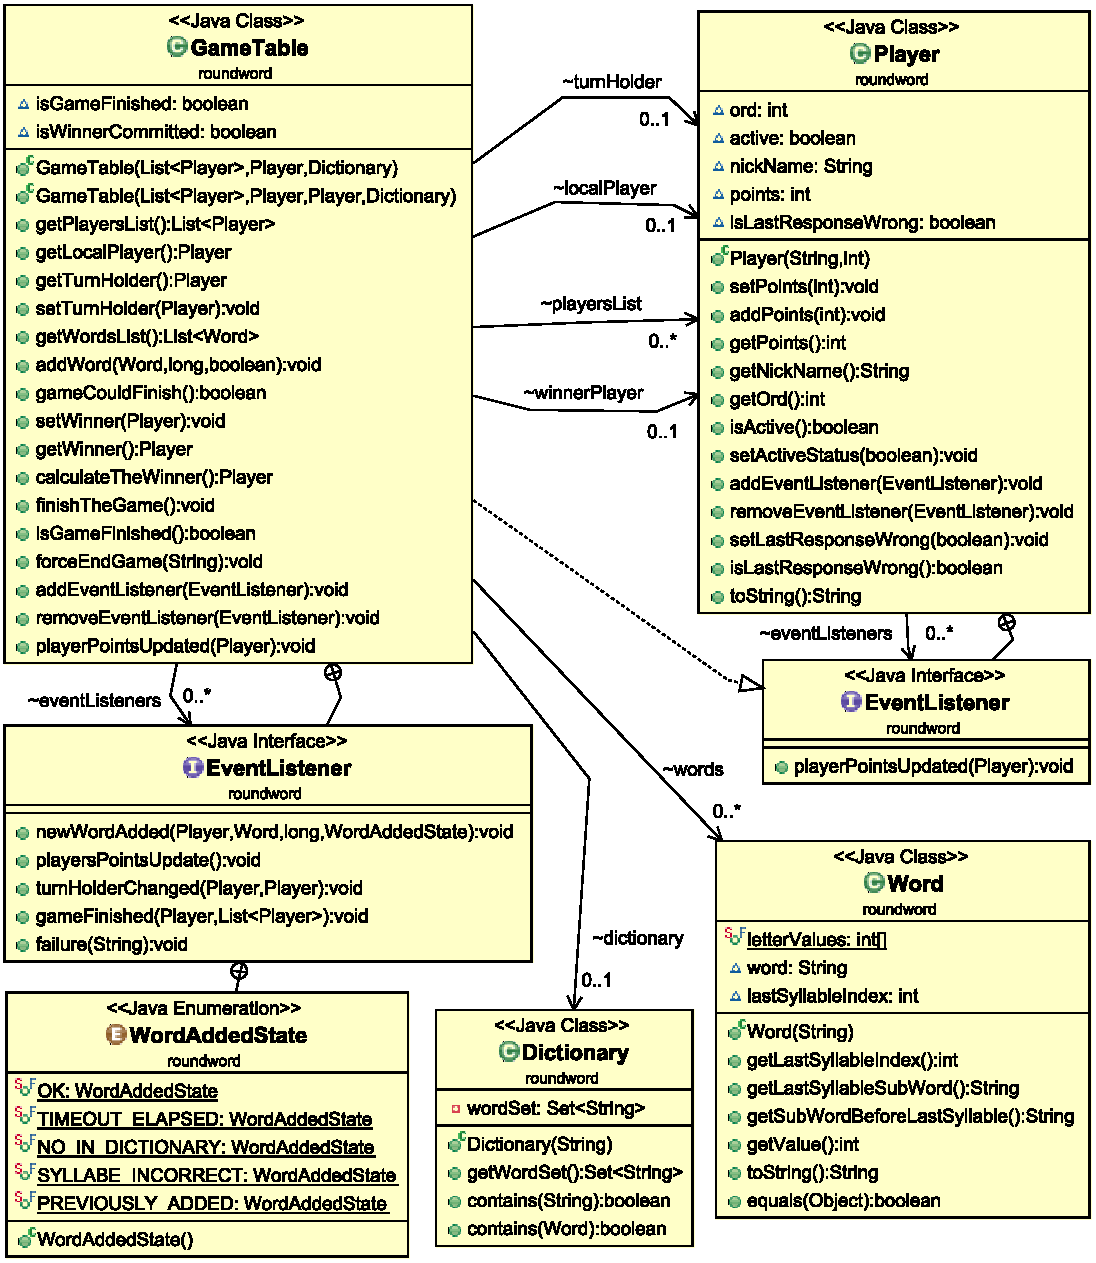
\includegraphics[scale=0.95]{imgs/ClassDiagram1.pdf}
		\label{fig:class_diagram1}
		\caption{Il diagramma delle classi di tutta la parte di modellazione del gioco, escludendo quindi tutte le classi per far partire il gioco, le classi di comunicazione, le classi per i giocatori automatici, e le classi per l'interfaccia con l'utente.}
	\end{center}
\end{figure}

In figura \ref{fig:class_diagram1} possiamo osservare il diagramma delle classi di tutta la parte di modellazione del gioco. Questa, come si può intuire, comprende solamente una piccola parte dell'intera applicazione. che corrisponde agli elementi che abbiamo cercato di descrivere in maniera approfondita. Da notare che anche il \texttt{Player} può generare un evento (che avviene al cambio del punteggio), ma questi vengono esclusivamente intercettati dal \texttt{GameTable} che a sua volta genera l'evento \texttt{playerPointsUpdate()}. Quest'ultimo serve solamente alla parte dell'interfaccia per aggiornare visivamente il punteggio dei giocatori.

\subsubsection{Comunicazione}

\begin{figure}
	\begin{center}
		\hspace*{-0.2in}
		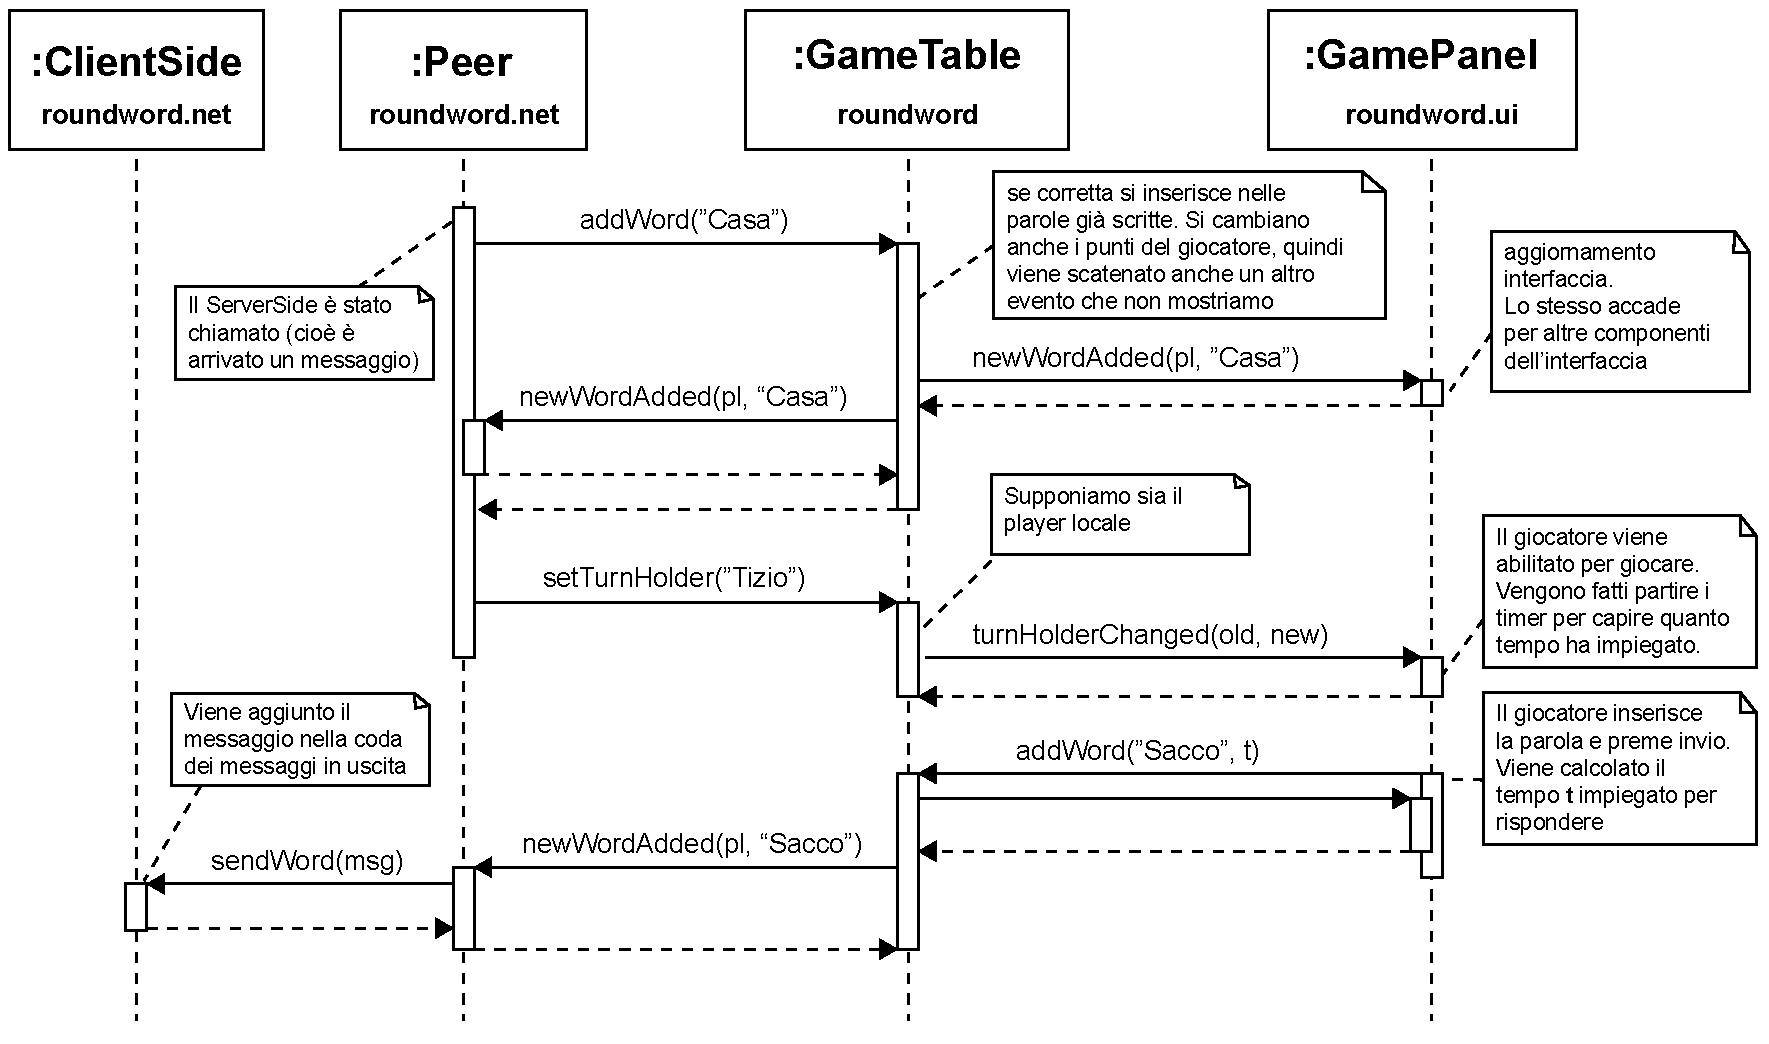
\includegraphics[scale=0.55]{imgs/Sequence1.pdf}
		\label{fig:sequence1}
		\caption{}
	\end{center}
\end{figure}	


Come abbiamo già discusso precedentemente, il \texttt{Peer} è un entità che controlla un determinato giocatore (\texttt{Player}). Esso, al momento della creazione di un gioco, si registra come listener per intercettare gli eventi del \texttt{GameTable}. Fatto ciò, ogni volta che l'utente locale ad esempio inserisce una parola, crea un messaggio di tipo \texttt{WordMsg} e lo aggiunge alla coda dei messaggi di uscita del \texttt{ClientSide} chiamando il metodo \texttt{send\_msg()}.

Il \texttt{ClientSide} è un thread con metodi e campi in più rispetto ad un normale thread, nasce e muore insieme al peer, provvedendo alla gestione dell'invio dei messaggi del peer. Si compone di una coda: è stato deciso di utilizzare la \texttt{BlockingQueue}, ma senza limitazioni nella dimensione, per fornire una coda che potesse essere utilizzata da più thread (il thread del peer e quello del \texttt{ClientSide}). Il metodo \texttt{send\_msg\_rmi(Msg)} altro non fa che ``eseguire'' il messaggio, raccogliendo tutti gli eventuali errori che possono essere generati da Java RMI. 

Utilizziamo il termine ``eseguire'' poiché un messaggio, in generale, è in realtà una classe che contiene un metodo \texttt{execute()} che chiama il metodo remoto presente nel server side del peer destinatario. Ogni tipo di messaggio esegue quindi un metodo differente, e i parametri del messaggio vengono utilizzati come argomenti per i metodi che vengono richiamati. 

Il \texttt{ServerSide} è invece una classe, istanziata solamente una volta per ogni peer, che costituisce l'insieme dei metodi che possono essere richiamati da ogni messaggio. Facendo un esempio, il metodo \texttt{execute()}, del messaggio di tipo \texttt{WordMsg}, esegue il metodo del \texttt{ServerSide} del destinatario chiamato \texttt{word()}, specificando come argomenti quelli propri del messaggio: chi lo ha generato (chi detiene il turno), la parola inserita, il tempo impiegato per inserire la parola, se esiste un vincitore (cioè la partita può terminare), e la lista dei peer morti che si sono accumulati lungo il percorso.

Nel seguente estratto, molto semplificato, del codice del \texttt{ClientSide} possiamo vedere quali siano le azioni base intraprese dal metodo \texttt{execute()} di un messaggio di tipo \texttt{WordMsg}.
\begin{verbatim}
	registry = LocateRegistry.getRegistry(destPeer.IPaddr, destPeer.serverPortno);
	stub = registry.lookup("ServerSide");
	response = stub.word(id, word, time, winnerId, crashedPeer);
\end{verbatim}

In figura \ref{fig:sequence1} possiamo osservare il comportamento della parte di comunicazione, messo in relazione con tutta la parte di modellazione del gioco. Le classi dell'interfaccia mostrate nel diagramma non sono state menzionate poiché inutili ai fini del progetto di sistemi distribuiti, possiamo solamente dire che il \texttt{GamePanel} è una componente dell'interfaccia che si occupa di inserire le parole da parte dell'utente.

\begin{figure}
	\vspace*{-0.5in}
	\begin{center}
		\hspace*{-0.45in}
		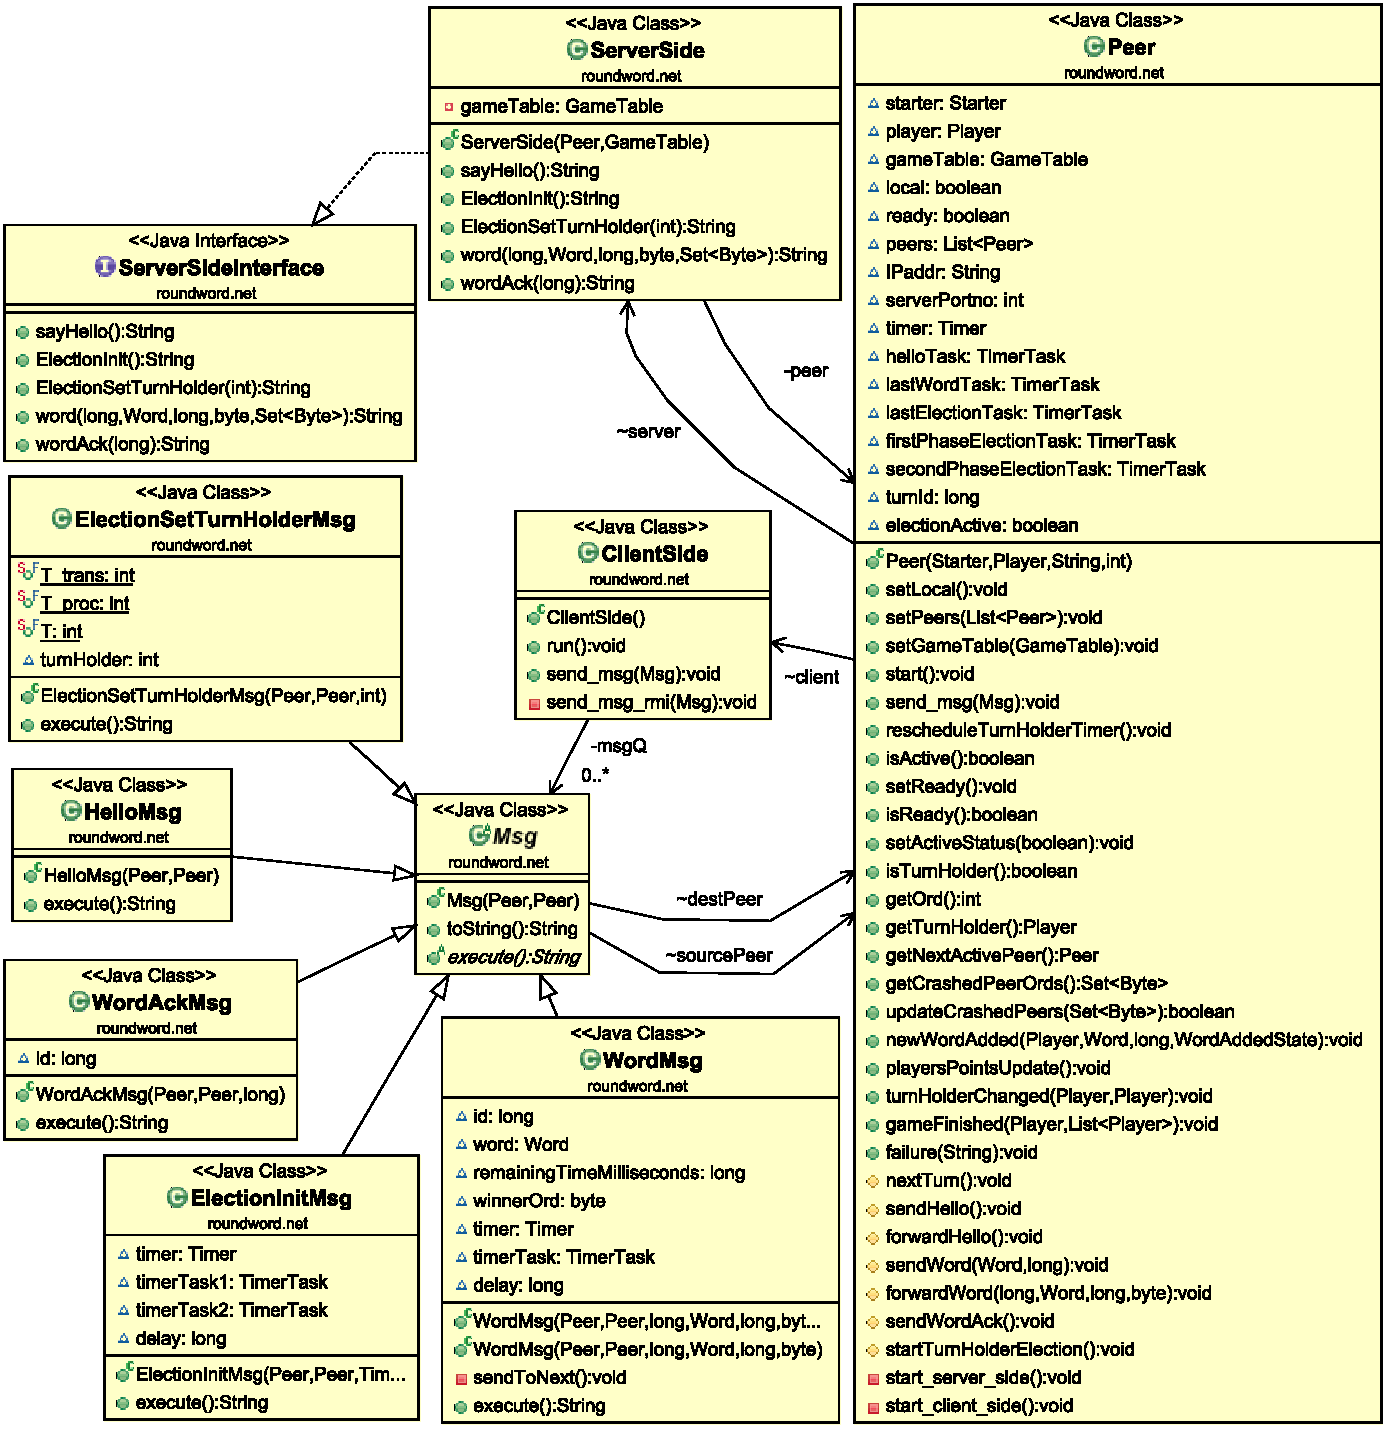
\includegraphics[scale=0.75]{imgs/ClassDiagram2.pdf}
		\label{fig:class_diagram2}
		\caption{Il diagramma delle classi di tutta la parte di comunicazione del gioco. Da notare \texttt{ServerSideInterface} che estende la classe \texttt{Remote}, e quindi viene solamente utilizzata per Java RMI, in modo che i client side dei vari peer possano chiamare in remoto i metodi del \texttt{ServerSide}.}
	\end{center}
\end{figure}

Il \texttt{ClientSide} ed il \texttt{ServerSide}, come anche il \texttt{Peer} vengono eseguiti in thread differenti. Detto ciò è stato molto importante gestire la concorrenza, sopratutto quando vengono modificati i campi del \texttt{Peer}. In particolare sono stati utilizzati i meccanismi di locking messi a disposizione da Java, per garantire che nessun thread potesse compiere delle operazioni contemporaneamente sul peer. Questa decisione non è limitante in termini di efficienza, poiché tali sono stati fatti in modo da non comprendere i ritardi di trasmissione della rete, ma solamente in modo da comprendere solamente le piccole porzioni che modificano o leggono i valori del peer.

Per quanto riguarda invece l'implementazione dei timeout, è stata utilizzata la classe messa a disposizione da Java, chiamata \texttt{Timer}. Questa, memorizzata all'interno del \texttt{Peer}, provvede ad eseguire determinate task dopo un certo periodo di tempo. Tali task (chiamati da Java \texttt{TimerTask}) possono comunque essere annullati, ad esempio in seguito ad una ricezione di un messaggio. Ogni task viene comunque memorizzato all'interno del \texttt{Peer} stesso, in modo che ogni metodo (del \texttt{Peer}, \texttt{ClientSide} o \texttt{ServerSide}) possa crearli, e salvandoli abbiamo la possibilità (anche da parte di altri metodi) di poterli annullare. I task utilizzati sono i seguenti:

\begin{itemize}
\item \texttt{helloTask}: per catturare il fatto che il messaggio \textit{hello} non è ritornato indietro.
\item \texttt{lastWordTask}: per catturare la morte dei forwarder del messaggio \textit{word}.
\item \texttt{lastElectionTask}: per catturare la morte del peer che detiene il turno attuale.
\item \texttt{firstPhaseElectionTask}: per catturare la morte dei peer candidati durante l'elezione.
\item \texttt{secondPhaseElectionTask}: per catturare la morte del peer eletto nella seconda fase dell'elezione.
\end{itemize}

Ognuno di questi viene creato e distrutto in momenti differenti. Ad esempio \texttt{lastWordTask} viene creato al momento dell'invio di un messaggio di \textit{word}, e ricreato quando invece si riceve un nuovo messaggio.

TODO: altro?

\section{Valutazione}
% confronto delle soluzioni proposte con soluzioni analoghe allo stato dell'arte.

Il gioco che è stato implementato segue le caratteristiche del classico gioco che ha avuto tanto successo, chiamato \textit{Ruzzle}, versione virtuale del noto gioco \textit{Il Paroliere}. Quest'ultimo, molto semplice, si basa anch'esso sulla conoscenza approfondita del vocabolario italiano, viene giocato da più giocatori, e costituisce quindi una sfida da parte del giocatore che in caso di vittoria lo induce a credere di essere un buon conoscitore della lingua italiana, e di conseguenza aumenta lo stimolo da parte dello stesso. Allo stesso modo si è pensato quale potesse essere un gioco con le stesse caratteristiche, che potesse essere anche implementato come progetto per questo corso di Sistemi Distribuiti. Tale gioco è molto citato nei libri ed in giro per il Web, ma viene pressoché giocato senza l'ausilio di un computer, o comunque senza l'ausilio di un entità completamente automatica che controlli la validità delle parole (ad esempio si utilizzano dei forum con dei moderatori umani). Questo probabilmente perché è molto difficile riuscire a costruire un algoritmo che faccia una sillabazione perfetta, per via delle tante eccezioni che sono presenti. Per questo motivo è già stato un passo avanti riuscire ad creare qualcosa di innovativo in questo senso, riuscendo a superare tali difficoltà.

TODO: Valutazioni a livello di comunicazione?

\section{Conclusioni}
% commenti conclusivi su possibili miglioramenti di quanto discusso, e possibili linee di intervento futuro.

TODO: ...

Sarebbe interessante portare avanti questo progetto anche in ambiente mobile, dove sicuramente un gioco simile può avere successo. Per quanto riguarda la giocabilità ci sono diverse proposte e migliorie. Prima di tutto potrebbe essere più divertente creare dizionari divisi per sezioni, in modo da limitare l'inserimento delle parole solamente a quelle di una determinata categoria scelta all'inizio del gioco. Inoltre, sarebbe interessante, in seguito ad uno studio di usabilità decidere se prevedere casi di terminazione che potrebbero divertire di più i giocatori, come ad esempio la vittoria di un giocatore che realizza moltissimi punti con una sola parola. Poi potrebbe essere anche utile sfruttare tutta la parte già realizzata dei giocatori automatici per rimpiazzare i giocatori che hanno avuto un crash.


% Bibliography
\bibliographystyle{ACM-Reference-Format-Journals}
\bibliography{riferimenti}


\end{document}
% End of v2-acmlarge-sample.tex (March 2012) - Gerry Murray, ACM
